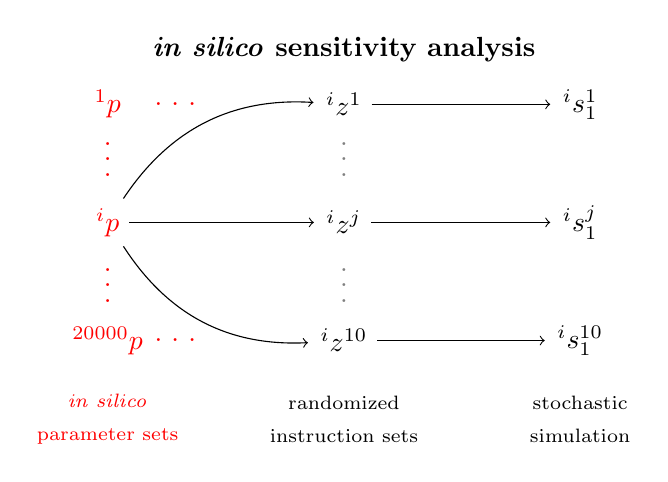
\begin{tikzpicture}[shorten >=1pt, auto]
\node[align=center] at (3,2.2) {\textbf{\textit{in silico} sensitivity analysis}};
  \node[]         (e1) at (0,1.5)    {\color{red} $\leftidx{^{1}} p$};
  \node[]         (e2) at (0,0)      {\color{red} $\leftidx{^{i}} p $};
  \node[]         (e3) at (0,-1.5)   {\color{red} $\leftidx{^{20000}} p$};

%% Fake Dots
  \node[] (f01)  at (0,1)    {\color{red}.};
  \node[] (f02)  at (0,0.8)  {\color{red}.};
  \node[] (f03)  at (0,0.6)  {\color{red}.};
  \node[] (f11)  at (0,-1)   {\color{red}.};
  \node[] (f12)  at (0,-0.8) {\color{red}.};
  \node[] (f13)  at (0,-0.6) {\color{red}.};

  \node[] (f01)  at (3,1)     {\color{gray}.};
  \node[] (f02)  at (3,0.8)   {\color{gray}.};
  \node[] (f03)  at (3,0.6)   {\color{gray}.};
  \node[] (f11)  at (3,-1)    {\color{gray}.};
  \node[] (f12)  at (3,-0.8)  {\color{gray}.};
  \node[] (f13)  at (3,-0.6)  {\color{gray}.};
   \node[] (f21)  at (.8,1.5) {\color{red}~.~.~.};
  \node[] (f31)  at (.8,-1.5) {\color{red}~.~.~.};



  \node[] (o1)  at (0,0)  {};
  
  \node[] (d1)  at (3,1.5)  {$\leftidx{^{i}} z ^{1}$};
  \node[] (d2)  at (3,0.0)  {$\leftidx{^{i}} z ^{j}$};
  \node[] (d3)  at (3,-1.5) {$\leftidx{^{i}} z ^{10}$};
  
  \node[] (b1)  at (6,1.5)  {$\leftidx{^{i}} s ^{1}_1$};
  \node[] (b2)  at (6,0.0)  {$\leftidx{^{i}} s ^{j}_1$};
  \node[] (b3)  at (6,-1.5) {$\leftidx{^{i}} s ^{10}_1$};


  \path[->]  (e2)  edge   [bend left=30]    (d1);
  \path[->]  (e2)  edge       (d2);
  \path[->]  (e2)  edge   [bend right=30]    (d3);
  
  \path[->]  (d1)  edge                    (b1);
  \path[->]  (d2)  edge                    (b2);
  \path[->]  (d3)  edge                    (b3);


   \node[align=center] at (0,-2.5) {\scriptsize\color{red} \textit{in silico}\\ \scriptsize \color{red}parameter sets};
  \node[align=center] at (3,-2.5) {\scriptsize randomized \\ \scriptsize instruction sets};
  \node[align=center] at (6,-2.5) {\scriptsize stochastic \\\scriptsize simulation};
\end{tikzpicture}

